% Compact single-column TikZ source for the evidence-first cascade (IV paper, Fig. 2).
% Build: tectonic fig_cascade.tex  -> fig_cascade.pdf   (latencies: measured p50 at 480 px, 2B)
\documentclass[tikz,border=2pt]{standalone}
\usepackage{mathptmx}
\usepackage{amsmath}
\usetikzlibrary{positioning,arrows.meta,calc,shapes.geometric}

\begin{document}
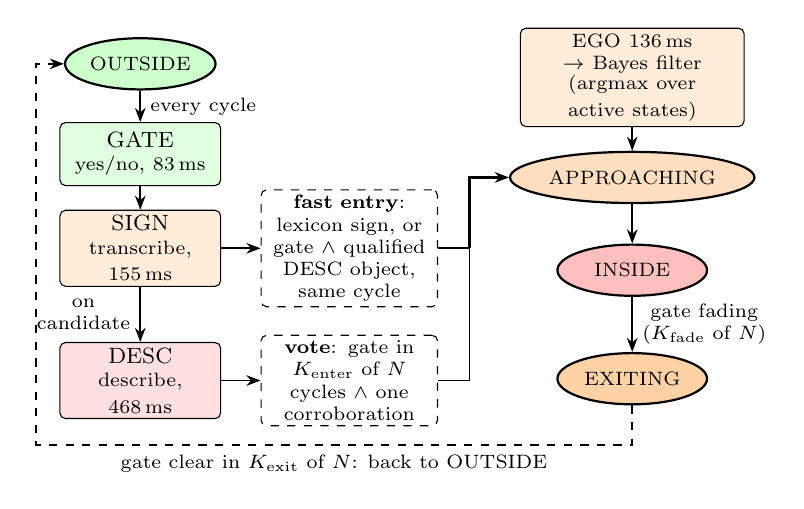
\begin{tikzpicture}[
  font=\footnotesize,
  chan/.style={draw, rounded corners=2pt, minimum height=8mm, text width=19mm, align=center, inner sep=2pt},
  cheap/.style={chan, fill=green!12},
  mid/.style={chan, fill=orange!15},
  costly/.style={chan, fill=red!12},
  state/.style={draw, ellipse, minimum height=6.5mm, minimum width=19mm, inner sep=1pt, align=center, thick, font=\scriptsize},
  arr/.style={-{Stealth[length=1.8mm]}, semithick},
  lab/.style={font=\scriptsize, align=center},
  door/.style={draw, rounded corners=2pt, dashed, text width=21mm, align=center, font=\scriptsize, inner sep=2pt}
]
% channels (left column)
\node[state, fill=green!20] (outside) {OUTSIDE};
\node[cheap, below=4mm of outside] (gate) {GATE\\[-1pt]\scriptsize yes/no, 83\,ms};
\node[mid, below=3mm of gate] (sign) {SIGN\\[-1pt]\scriptsize transcribe, 155\,ms};
\node[costly, below=7mm of sign] (desc) {DESC\\[-1pt]\scriptsize describe, 468\,ms};
\draw[arr] (outside) -- node[lab, right] {every cycle} (gate);
\draw[arr] (gate) -- (sign);
\draw[arr] (sign) -- node[lab, left] {on\\candidate} (desc);

% entry doors (middle column), level with SIGN and DESC
\node[door, right=5mm of sign] (fast) {\textbf{fast entry}: lexicon sign, or gate $\wedge$ qualified DESC object, same cycle};
\node[door, right=5mm of desc] (vote) {\textbf{vote}: gate in $K_\text{enter}$ of $N$ cycles $\wedge$ one corroboration};
\draw[arr] (sign.east) -- (fast.west);
\draw[arr] (desc.east) -- (vote.west);

% active states (right column)
\node[state, fill=orange!25, right=9mm of fast, yshift=9mm] (appr) {APPROACHING};
\node[state, fill=red!25, below=5mm of appr] (inside) {INSIDE};
\node[state, fill=orange!35, below=7mm of inside] (exiting) {EXITING};
\coordinate (J) at ($(fast.east)+(4mm,0)$);
\draw[semithick] (fast.east) -- (J);
\draw[semithick] (vote.east) -| (J);
\draw[arr, thick] (J) |- (appr.west);
\draw[arr] (appr) -- (inside);
\draw[arr] (inside) -- node[lab, right] {gate fading\\($K_\text{fade}$ of $N$)} (exiting);

% ego + filter
\node[mid, above=3mm of appr, text width=27mm, minimum height=5mm] (ego) {\scriptsize EGO 136\,ms $\to$ Bayes filter\\[-2pt]\scriptsize (argmax over active states)};
\draw[arr] (ego) -- (appr);

% exit back to outside
\draw[arr, dashed] (exiting.south) -- ++(0,-5mm) -| node[lab, below, pos=0.25] {gate clear in $K_\text{exit}$ of $N$: back to OUTSIDE} ($(desc.south west)+(-3mm,0)$) |- (outside.west);
\end{tikzpicture}
\end{document}
